    
\documentclass[11pt]{article}
\usepackage{times}
\usepackage{graphicx}
\usepackage[format=plain,labelfont={bf,it},textfont=it,tableposition=above]{caption}
    \usepackage{fullpage}
    
    \title{Keep Your Distance! Real-time Social Distancing Using Wearable ESP32s}
    \author{Ryan Williamson - 2306841w}

    \begin{document}
    \maketitle
    
    
     

\section{Status report}

\subsection{Proposal}\label{proposal}

\subsubsection{Motivation}\label{motivation}

A real-time proximity sensor configurable for the various distances recommended 
for social distancing allows for users, particularly office / retail 
workers, to feel more comfortable that they are staying as safe as 
possible from SARS-CoV-2. This could also be applicable to unknown 
future pandemics to help reduce initial impacts.

\subsubsection{Aims}\label{aims}

This project will develop a system involving two components, an 
Android app, and an ESP32 micro-controller. The ESP32 will detect 
other so configured ESP32 devices and alert the user, while also 
logging this interaction to the companion app. Both the device-device 
and phone-device connections will be implemented using Bluetooth Low 
Energy (BLE).

\subsection{Progress}\label{progress}

\begin{itemize}
    \setlength\itemsep{0.1em}
\item Languages chosen for both Android App (Java), and ESP32 (C++ after switching
from Micropython).
\item Seven papers summarised, with a partial literature review created to link 
five of the papers together.
\item User stories, personas, and scenarios created.
\item  MOSCOW requirements specification created.
\item  Very rough dissertation structure outlined.
\item  Interference vectors considered and documented.
\item  Bluetooth protocol between devices and device to app created and visualised.
\item  Prototype app and device created to implement initial BLE stack, as well
as allow for an experiment to be conducted.
\item  Experiment conducted to get 250 RSSI values at 5 distances, incremented at 
0.5 metres.
\item  Parameter space exploration conducted on experiment data to get best fit 
values for measured power and environment factor. As shown in Figure \ref{fig:rssi_experiment_graph}.

\end{itemize}

\begin{figure}[!ht]
    \centering
    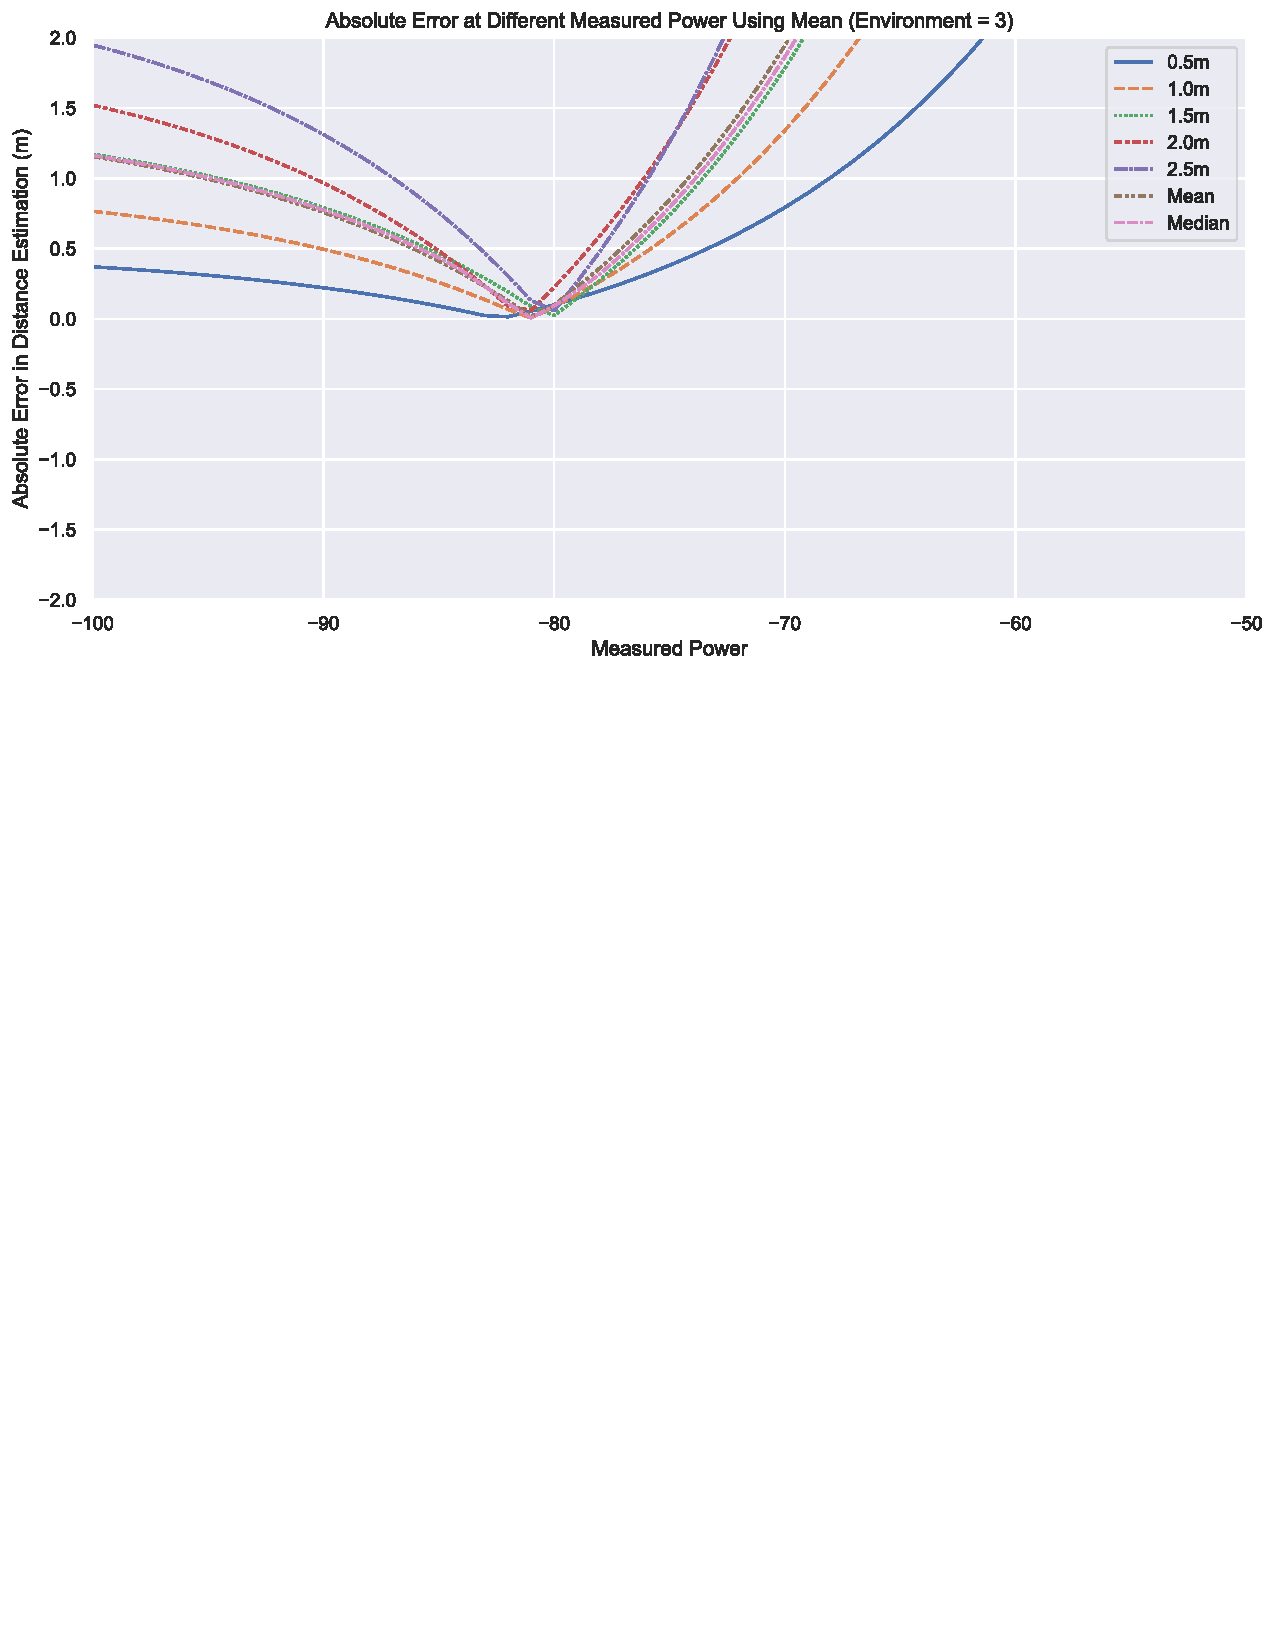
\includegraphics[width=0.85\linewidth]{../images/pdf/rssi_experiment_graph.pdf}
    
    \caption{
      ``A line graph showing the absolute error of the calculated distance vs the 
      actual distance for different values of measured power. Environment=3 was 
      chosen as best. Finding best measured power is where all lines here are 
      as close to zero as possible.''
    }
    
    % use the notation fig:name to cross reference a figure
    \label{fig:rssi_experiment_graph}
\end{figure}

\subsection{Problems and risks}\label{problems-and-risks}

\subsubsection{Problems}\label{problems}

The following issues were encountered in the project so far.

\begin{itemize}
    \setlength\itemsep{0.1em}
\item Micropython BLE functionality still in development and was not suitable for 
the project. This meant there was a lot of work in Micropython in the beginning that 
had to be replicated in Arduino C++.
\item Android Bluetooth libraries very low level, so it took quite some time to get 
the app BLE functionality working.
\item Not much documentation of the esp32 BLE library, so took quite a lot of digging
and reading source code to get it working.
\item Current BLE scanning method is not secure - will need to be replaced.

\end{itemize}

\subsubsection{Risks}\label{risks}

The following are potential issues I see coming up.

\begin{itemize}
    \setlength\itemsep{0.1em}
\item Lack of real user evaluation due to COVID. \textbf{Mitigation}: will consider 
alternate styles of evaluation to supplment limited hands-on evaluation.
\item RSSI values are quite inconsistent. \textbf{Mitigation}: Look into an 
algorithm, such as a sliding window based one, to look at the past n readings. As 
opposed to a simple threshold.
\item Can't figure out how to store data in non-volatile on esp 32. 
\textbf{Mitigation}: Currently just sending data to phone, but would like to try and 
find a solution to prevent data loss on the device for an extra layer of redundancy.

\end{itemize}

\subsection{Plan}\label{plan}

\begin{itemize}
    \setlength\itemsep{0.1em}
    \item
      Week 1-2: Finalise and begin to send out user surveys, and perform experiments 
      with users. \textbf{Deliverable: Raw data, and experiment results.}
    \item
      Week 3-4: Analyse user evaluations and experiments to draw conclusions about
      system accuracy, efficiency, and usability. \textbf{Deliverable: Some graphs 
      and conclusions.}
    \item
      Week 5-7: Write up. \textbf{Deliverable: First draft submitted to
      Jeremy.}
    \item
      Week 8-9: Write up - Second Draft. \textbf{Deliverable: Second draft submitted to
      Jeremy.}
    \item
      Week 10: Final polish on dissertation. \textbf{Deliverable: Final changes checked 
      over by Jeremy, then submitted via Moodle.}
    \end{itemize}

    
\subsection{Ethics and data}\label{ethics}

I have verified that the ethics checklist will apply to surveys I need to do. I will sign and complete the checklist.
I have sought ethical guidance from the School's ethics convener, as I need to use non-standard hardware (ESP32).


\end{document}
